% ****** Start of file apssamp.tex ******
%
%   This file is part of the APS files in the REVTeX 4.1 distribution.
%   Version 4.1r of REVTeX, August 2010
%
%   Copyright (c) 2009, 2010 The American Physical Society.
%
%   See the REVTeX 4 README file for restrictions and more information.
%
% TeX'ing this file requires that you have AMS-LaTeX 2.0 installed
% as well as the rest of the prerequisites for REVTeX 4.1
%
% See the REVTeX 4 README file
% It also requires running BibTeX. The commands are as follows:
%
%  1)  latex apssamp.tex
%  2)  bibtex apssamp
%  3)  latex apssamp.tex
%  4)  latex apssamp.tex
%
\documentclass[%
 reprint,
superscriptaddress,
%groupedaddress,
%unsortedaddress,
%runinaddress,
%frontmatterverbose, 
%preprint,
%showpacs,preprintnumbers,
%nofootinbib,
%nobibnotes,
%bibnotes,
 amsmath,amssymb,
 aps,
%pra,
prb,
%rmp,
%prstab,
%prstper,
%floatfix,
]{revtex4-1}
\usepackage{amsmath}
\newcommand*\diff{\mathop{}\!\mathrm{d}}
\newcommand*\Diff[1]{\mathop{}\!\mathrm{d^#1}}
\usepackage{graphicx}
\usepackage{soul}
\usepackage{mhchem, textcomp}
\usepackage{graphicx}% Include figure files
\usepackage{dcolumn}% Align table columns on decimal point
\usepackage{bm}% bold math
\usepackage{wrapfig}
\usepackage{graphicx, type1cm, lettrine}
% Uncomment the following two lines to force Latex to place the figure.
% Use [H] when including graphics. Note 'H' instead of 'h'
\usepackage{float}
\usepackage{booktabs}
\restylefloat{figure}
\usepackage{hyperref}
\usepackage{array}
\newcolumntype{P}[1]{>{\centering\arraybackslash}p{#1}}% add hypertext capabilities
%\usepackage[mathlines]{lineno}% Enable numbering of text and display math
%\linenumbers\relax % Commence numbering lines
%\usepackage[showframe,%Uncomment any one of the following lines to test 
%%scale=0.7, marginratio={1:1, 2:3}, ignoreall,% default settings
%%text={7in,10in},centering,
%%margin=1.5in,
%%total={6.5in,8.75in}, top=1.2in, left=0.9in, includefoot,
%%height=10in,a5paper,hmargin={3cm,0.8in},
%]{geometry}

\begin{document}

\preprint{APS/123-QED}

\title{Photoresponsivity enhancement in monolayer MoS$_2$ phototransistors by rapid O$_2$:Ar plasma treatment}% Force line breaks with \\

\author{Jakub Jadwiszczak}
\affiliation{School of Physics, Trinity College Dublin, Dublin 2, Ireland}
\affiliation{Centre for Research on Adaptive Nanostructures and Nanodevices (CRANN), Trinity College Dublin, Dublin 2, Ireland} 
\affiliation{Advanced Materials and BioEngineering Research Centre (AMBER), Trinity College Dublin, Dublin 2, Ireland}

\author{Gen Li}
\affiliation{School of Physics, Trinity College Dublin, Dublin 2, Ireland}
\affiliation{Centre for Research on Adaptive Nanostructures and Nanodevices (CRANN), Trinity College Dublin, Dublin 2, Ireland} 
\affiliation{Advanced Materials and BioEngineering Research Centre (AMBER), Trinity College Dublin, Dublin 2, Ireland}

\author{Darragh Keane}
\affiliation{Centre for Research on Adaptive Nanostructures and Nanodevices (CRANN), Trinity College Dublin, Dublin 2, Ireland} 
\affiliation{Advanced Materials and BioEngineering Research Centre (AMBER), Trinity College Dublin, Dublin 2, Ireland}
\affiliation{School of Chemistry, Trinity College Dublin, Dublin 2, Ireland}

\author{Conor P. Cullen}
\affiliation{School of Physics, Trinity College Dublin, Dublin 2, Ireland}
\affiliation{Centre for Research on Adaptive Nanostructures and Nanodevices (CRANN), Trinity College Dublin, Dublin 2, Ireland} 
\affiliation{Advanced Materials and BioEngineering Research Centre (AMBER), Trinity College Dublin, Dublin 2, Ireland}

\author{\\Jing Jing Wang}
\affiliation{Centre for Research on Adaptive Nanostructures and Nanodevices (CRANN), Trinity College Dublin, Dublin 2, Ireland} 

\author{Yangbo Zhou}
\affiliation{School of Physics, Trinity College Dublin, Dublin 2, Ireland}
\affiliation{Centre for Research on Adaptive Nanostructures and Nanodevices (CRANN), Trinity College Dublin, Dublin 2, Ireland} 
\affiliation{Advanced Materials and BioEngineering Research Centre (AMBER), Trinity College Dublin, Dublin 2, Ireland}
\affiliation{School of Material Science and Engineering, Nanchang University, 999 Xuefu Road, Nanchang, Jiangxi, China, 330031}

\author{Daniel S. Fox}
\affiliation{School of Physics, Trinity College Dublin, Dublin 2, Ireland}
\affiliation{Centre for Research on Adaptive Nanostructures and Nanodevices (CRANN), Trinity College Dublin, Dublin 2, Ireland} 
\affiliation{Advanced Materials and BioEngineering Research Centre (AMBER), Trinity College Dublin, Dublin 2, Ireland}

\author{\\Georg S. Duesberg}
\affiliation{Centre for Research on Adaptive Nanostructures and Nanodevices (CRANN), Trinity College Dublin, Dublin 2, Ireland} 
\affiliation{Advanced Materials and BioEngineering Research Centre (AMBER), Trinity College Dublin, Dublin 2, Ireland}
\affiliation{School of Chemistry, Trinity College Dublin, Dublin 2, Ireland}

\author{John J. Boland}
\affiliation{Centre for Research on Adaptive Nanostructures and Nanodevices (CRANN), Trinity College Dublin, Dublin 2, Ireland} 
\affiliation{Advanced Materials and BioEngineering Research Centre (AMBER), Trinity College Dublin, Dublin 2, Ireland}
\affiliation{School of Chemistry, Trinity College Dublin, Dublin 2, Ireland}

\author{Hongzhou Zhang}
\email{hozhang@tcd.ie}
\affiliation{School of Physics, Trinity College Dublin, Dublin 2, Ireland}
\affiliation{Centre for Research on Adaptive Nanostructures and Nanodevices (CRANN), Trinity College Dublin, Dublin 2, Ireland} 
\affiliation{Advanced Materials and BioEngineering Research Centre (AMBER), Trinity College Dublin, Dublin 2, Ireland}


% Collaboration name, if desired (requires use of superscriptaddress option in \documentclass). 
% \noaffiliation is required (may also be used with the \author command).
%\collaboration{}
%\noaffiliation
\begin{abstract}

The chemical modification of the surface of MoS$_2$ serves to alter the electrical properties of the material significantly. Here, we report the two-fold enhancement of the photoresponsivity of monolayer MoS$_2$ FETs by rapid treatment with O$_2$:Ar (1:3) plasma. We characterise the surface of plasma-exposed MoS$_2$ by TEM, AFM, Raman and PL mapping and uncover the role of MoO$_x$ in improving the photocurrent generation in our devices. Both photoresponsivity and field effect mobility are enhanced under illumination wavelengths of 488 nm and 632 nm, for a range of laser powers. The results highlight the beneficial effect of plasma-treatment as a fast and convenient way of modifying and improving the properties of 2D MoS$_2$ devices for future consideration in optoelectronics research.

\end{abstract}
\pacs{}% insert suggested PACS numbers in braces on next line

\maketitle %\maketitle must follow title, authors, abstract and \pacs

% Body of paper goes here. Use proper sectioning commands. 
% References should be done using the \cite, \ref, and \label commands


\lettrine[lines=2]{T}wo-dimensional materials have attracted wide research interest due to their intriguing physical properties and potential applications. In addition to graphene, the family of transition-metal dichalcogenides (TMDs) has emerged as the most studied group of 2D materials. The bandgap of TMDs ranges between 1.1-2.1 eV, \cite{wang2012electronics} which makes them good candidates for various applications; including photodetectors, \cite{Li2015, Miao2015, Qiu2014} field effect transistors (FETs), \cite{Radisavljevic2013} and logic devices.\cite{huang2013large} Molybdenum disulfide (MoS$_2$) is a typical layered TMD. The MoS$_2$ crystal is an indirect gap semiconductor with a band gap of 1.2 eV in the bulk, and a direct gap of 1.8 eV in the monolayer limit.\cite{Mak2010a} This allows monolayer MoS$_2$ FETs to achieve high ON/OFF current ratios ranging between 10$^7$-10$^9$ \cite{qiu2012electrical}, while preserving decent carrier mobility. 
Hence, optoelectronic devices fabricated from MoS$_2$ have received notable attention in recent years. \cite{LopezSanchez2013, Chen2015, qin2016atomic} MoS$_2$ phototransistors are easy to fabricate, respond to a wide range of excitation wavelengths,\cite{LopezSanchez2013, Wang2015}, exhibit sub-milisecond DC photoresponses \cite{yore2017large} and their photoresponsivity can be tuned by various methods. These include back-gating,\cite{Yin2012} encapsulation in HfO$_2$ \cite{Kufer2015}, strain engineering \cite{wang2017thermally} and evaporation of MoO$_x$ overlayer.\cite{Yoo2017}\\
\indent In this work, we demonstrate the enhancement of photoresponsivity of CVD monolayer MoS$_2$ phototransistors by rapid treatment with O$_2$:Ar (1:3) plasma. The photoresponsivity is improved two-fold after only 2 seconds of exposure to the plasma. At the same time, the field effect mobility of the monolayer FET under illumination improves by over one order of magnitude. We find that the improvement of electrical performance is due to the surface presence of MoO$_x$ resulting from chemical conversion of MoS$_2$ by the oxygen-containing plasma. This methodology presents a fast and convenient way to tune the optoelectronic performance of on-chip CVD-grown MoS$_2$. \newline
\indent Monolayer MoS$_2$ samples were synthesized on SiO$_2$/Si substrates using the CVD microreactor method previously reported \cite{Maria2014}. The flakes were identified by optical microscope and were further characterized using AFM and Raman spectroscopy to confirm the number of layers. Electrodes were fabricated by standard electron beam lithography, using poly(methyl methacrylate) 350K photoresist, baked at 180$^{\circ}$C for 3 minutes after spin coating, and then exposed at a dose of 130 $\mu$C/$\mu$m$^2$ with a 20 keV electron beam. Resist was developed in methyl isobutyl ketone:isopropyl alcohol (1:3) solution for 60 s, followed by an IPA rinse for 25 s and drying using a N$_2$ gun. Ti(10 nm)/Au(40 nm) contacts were deposited using an e-beam evaporation tool, followed by lift-off in acetone for 8 hours at room temperature. Plasma treatment was carried out in a Fischione Instruments 1020 plasma cleaner for 2 seconds, utilising O$_2$:Ar (1:3) gas, at a chamber base pressure of $\sim$ 5 mbar. The electrical characterization was performed in a two-probe configuration on a micromanipulator probe station (Imina miBot) using a source meter unit (Agilent B2912A) in the ambient. The devices were back-gated through the heavily p-doped Si substrate. The wavelengths of the lasers used for FET irradiation were 488 nm and 632 nm. For each wavelength, the power density was tuned at five different levels and pre-measured to ensure no power fluctuation throughout the experiment. The laser was directed through a condenser lens (20 $\times$, NA = 0.4) and the spot size was $\approx$ 1.5 $\mu$m and $\approx$ 1.9 $\mu$m for 488 nm and 632 nm respectively. Transmission electron microscopy (TEM) was carried out in a FEI Titan 80-300 system operated at 300 kV, at a chamber pressure of $4 \cdot 10^{-7}$ mbar. Monolayer samples were transferred onto TEM grids using the PMMA stamp transfer methodology previously described \citep{bie2011site}. Atomic force microscopy was performed at ambient pressure in an Oxford Asylum system using cantilevers calibrated at 140 kHz. Raman and photoluminescence spectra were acquired using a WITec Alpha 300 R confocal Raman microscope with an excitation wavelength of 532 nm. Raman spectra were acquired using a spectral grating with 1800 lines/mm, while a lower resolution grating with 600 lines/mm was used for detecting photoluminescence. A low laser power ($<$ 100 $\mu$W) was used to minimize any laser-induced damage or heating of the sample. \newline
\indent Our monolayer CVD MoS$_2$ device performs as a standard
n-type FET with a field effect mobility of 0.13 cm$^2$ V$^{-1}$ s$^{-1}$ under no illumination. We collected the output and transfer characteristics of the device under two different wavelengths (488 nm $\&$ 632 nm), at 5 different powers for each. The device channel was 3 $\mu$m, thus the laser spot avoided the Au electrodes during illumination and all of the collected photo-generated current originated in the MoS$_2$.\\


\begin{center}
\begin{figure}[!htb]
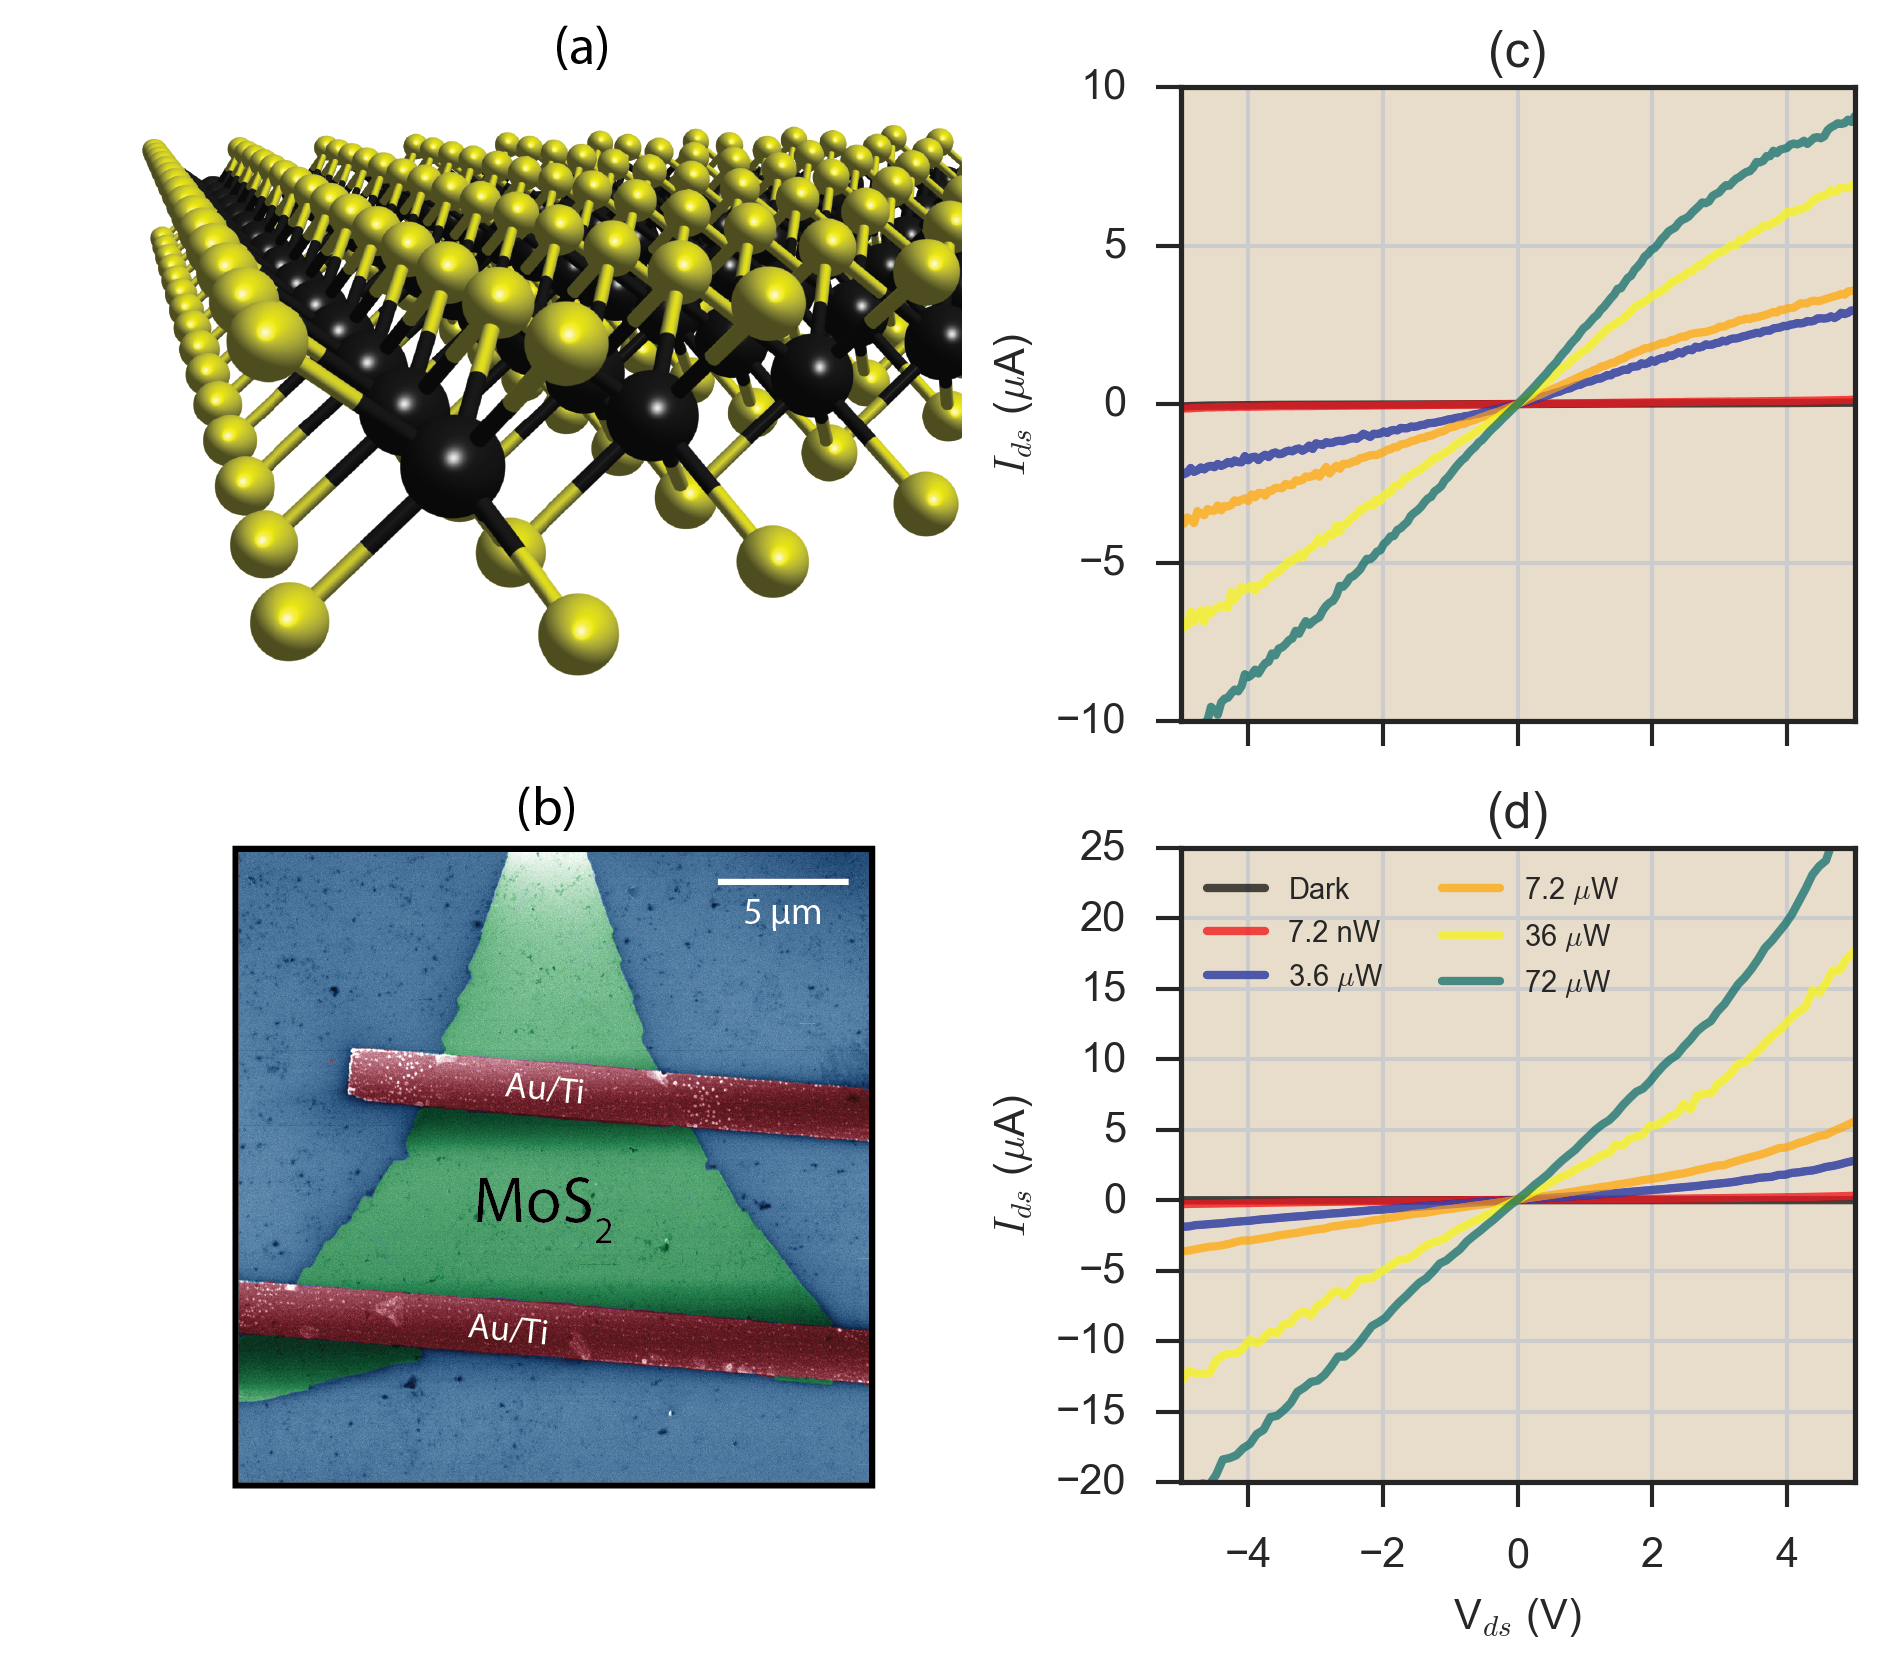
\includegraphics[width=80mm]{Fig_1}
\caption{FET characteristics under 632 nm laser illumination: (a) Output curve of the untreated single layer MoS$_2$ device, demonstrating a good Ohmic contact between the material and the metal electrode. Output current increases with increasing laser power. (b) Transfer characteristics of the same untreated device, demonstrating standard n-type  FET behaviour and increase of carriers in the channel at higher laser powers. (c) Post-plasma treatment IV curves show a similar trend with increasing laser power, but the output current has increased substantially for the same device. (d) Similarly, the level of current in the transfer curves of the plasma-exposed device has increased by one order of magnitude at higher laser powers.}
\end{figure}
\end{center}


\indent Figure 1 shows the output and transfer characteristics of the device under the 632 nm laser before and after plasma treatment. Comparing Figs. 1(a) and 1(c), it can be seen that the drain-source current increases two-fold for illuminated samples after 2 seconds of plasma exposure at the highest incident power. Figs. 1(b) and 1(d) show the transfer curves for the same sample, before and after plasma treatment. The threshold voltage of the untreated device is shifted drastically to the negative gate biases in curves obtained under higher power illumination. The associated inability to turn off the carrier-rich FET channel at standard gate biases is evident from the plots, where the output current stays firmly above 10$^{-7}$ A even at V$_{GS}$ =  - 60 V. After plasma treatment, the level of output current in the threshold region drops by close to 1 order of magnitude, while the onset voltage is seen to shift to more positive gate biases indicating oxygen-related p-type doping in the material \cite{giannazzo2017ambipolar,guo2017observation}. In addition, at low laser powers it can be seen that the MoS$_2$ now possesses a weak ambipolar response past the gate threshold, indicating hole conduction caused by the likely presence of plasma-created oxides \cite{chuang2014mos2, mcdonnell2014hole}. However, the output current in the saturation region of the gate curve has now improved by one order of magnitude under all illumination powers. The dark gated current has decreased slightly, indicating the necessity of illumination for performance improvement after plasma treatment.
\begin{center}
\begin{figure}[!htb]
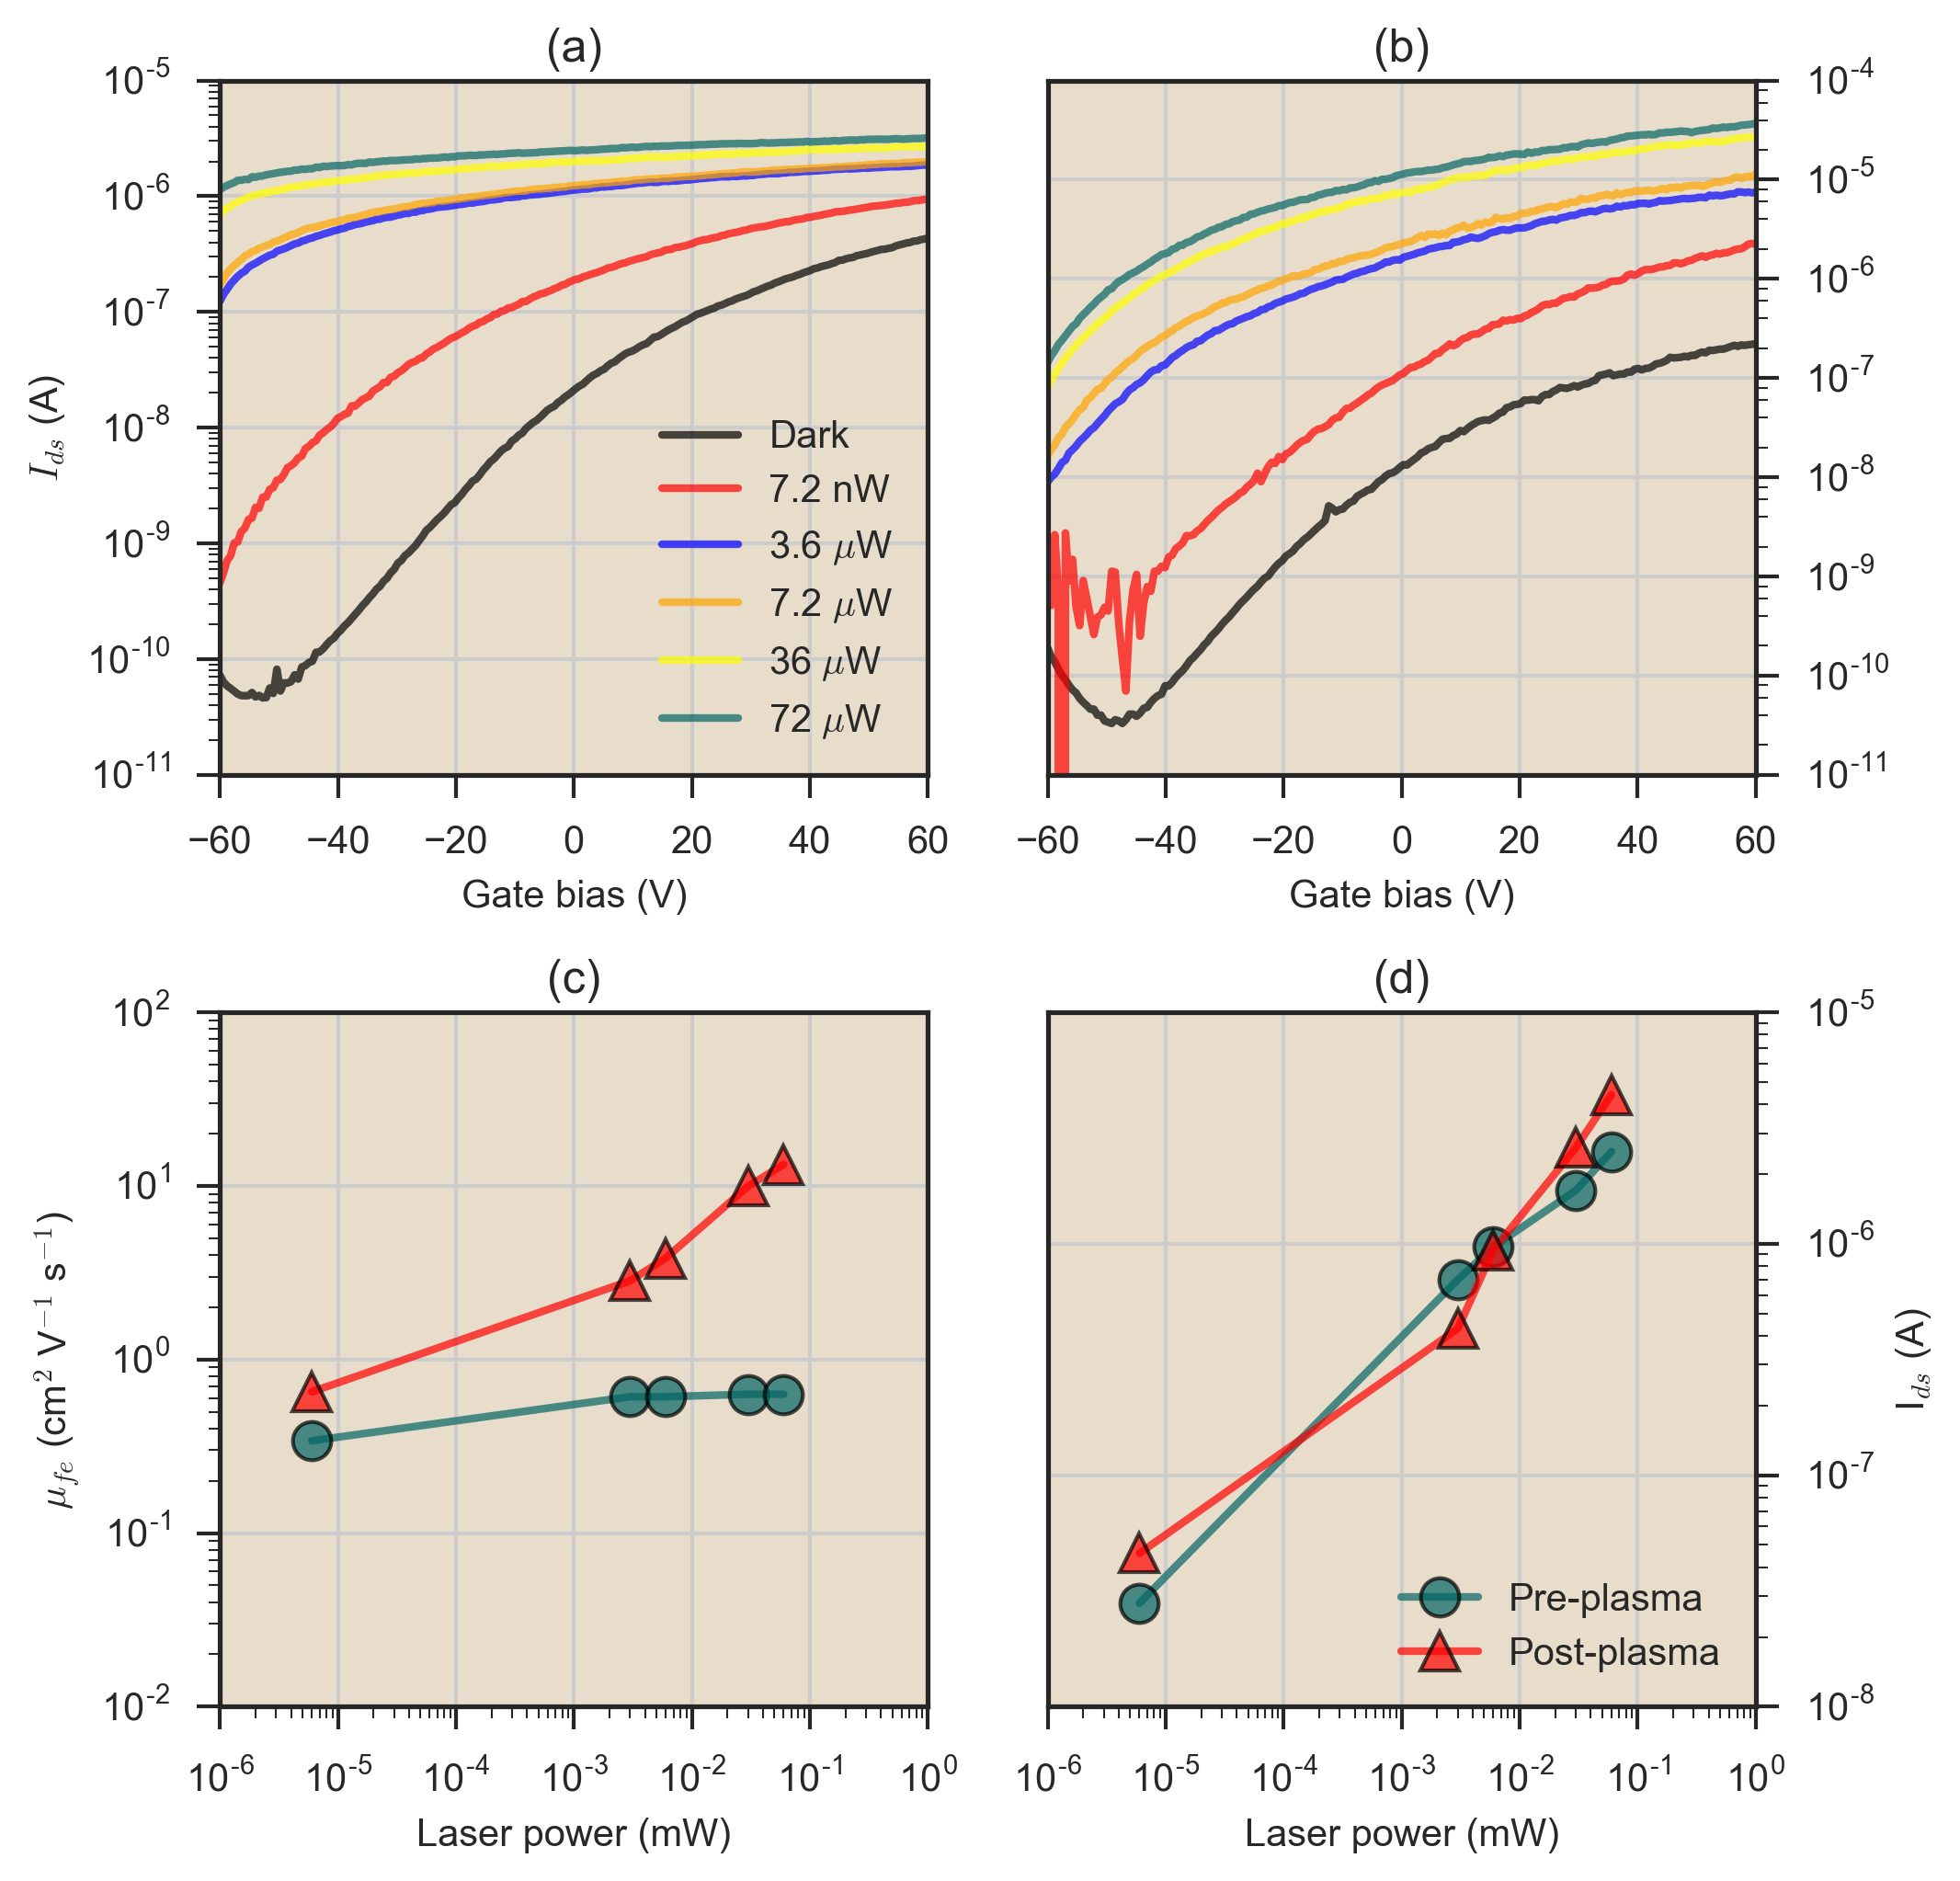
\includegraphics[width=80mm]{Fig_2.png}
\caption{The comparison of mobility and photocurrents before and after plasma treatment: (a) Mobility comparison before and after plasma treatment as a function of 488 nm laser power. (b) Photocurrent comparison before and after plasma exposure as a function of 488 nm laser power. (c) Mobility comparison before and after plasma treatment as a function of 488 nm laser power. (d) Photocurrent comparison before and after plasma exposure as a function of 488 nm laser power. Lines are guides to the eye.}
\end{figure}
\end{center}

\onecolumngrid

\begin{table}
\centering
\caption{Mobility and photoresponsivity at different illumination wavelengths before and after plasma treatment.}
\label{my-label}
\begin{tabular}{@{}ccccc@{}}
\toprule
                       & \multicolumn{2}{c}{488 nm} & \multicolumn{2}{c}{632 nm} \\ \hline \hline \\
\multicolumn{1}{c}{Plasma exposure time} &  $\mu_{fe}$ {\small (cm$^{2}$ V$^{-1}$ s$^{-1}$)}         &      R$_{ph}$ {\small (A/W)}     &    $\mu_{fe}$ {\small (cm$^{2}$ V$^{-1}$ s$^{-1}$) }      &    R$_{ph}$ {\small (A/W)}       \\ \hline \\
\multicolumn{1}{c}{0 seconds} &   0.95        &        x   &     0.63      &      0.04        \\ \hline \\
\multicolumn{1}{c}{2 seconds} &       13.5    &      x    & 13.3          &  0.4             \\ \hline
\end{tabular}
\end{table}

\twocolumngrid
\begin{center}
\begin{figure}[!htb]
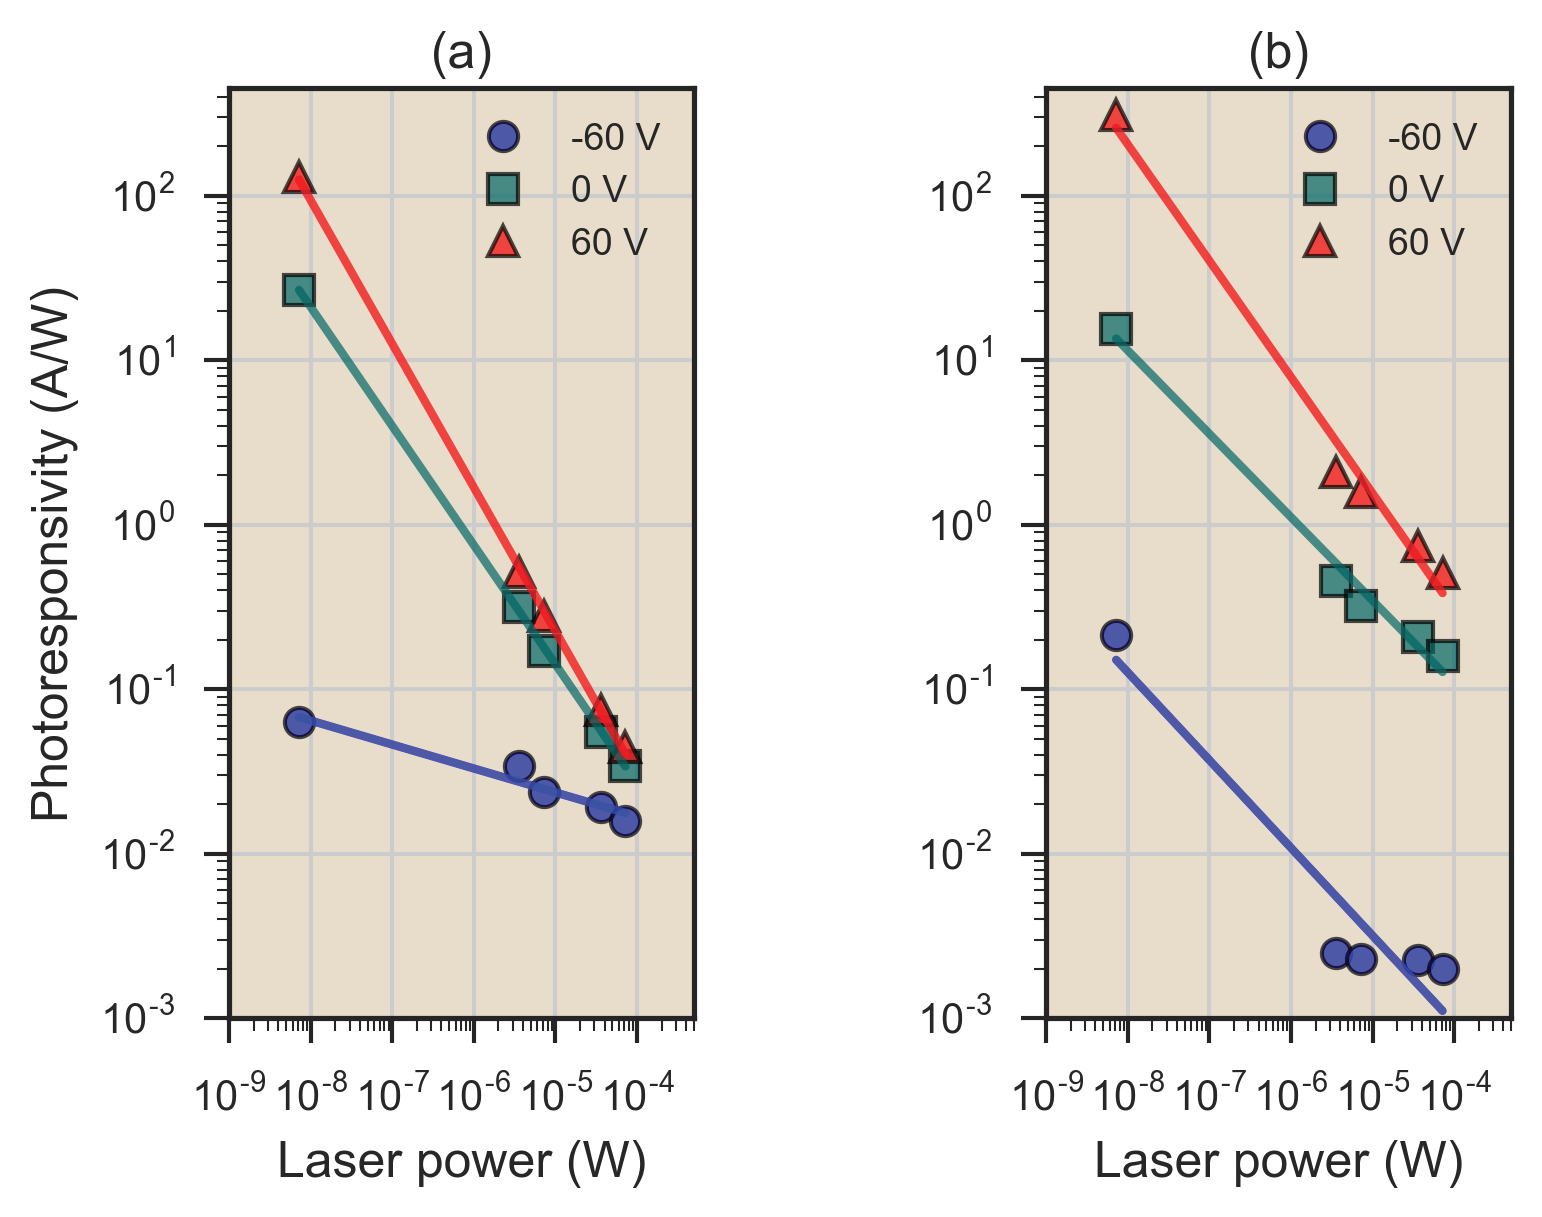
\includegraphics[width=80mm]{R_ph}
\caption{Photoresponsivity as a function of irradiation power extracted at gate voltages of - 60, 0 and 60 Volts: (a) Trends for the untreated MoS$_2$ sample. (b) Increased responsivity of the MoS$_2$ phototransistor after 2 seconds of O$_2$:Ar plasma treatment.}
\end{figure}
\end{center}
\indent Figures 2(a) and 2(c) track the MoS$_2$ channel field effect mobility ($\mu_{fe}$) before and after chemical reaction with the plasma, extracted at 488 nm and 632 nm respectively. Even with no laser illumination, the mobility is seen to improve in the plasma-treated samples by just under 1 order of magnitude, which has been explored in previous work \cite{jadwiszczak2017oxide}. When the device is exposed to the plasma for 2 seconds, the carrier mobility increases 10-fold with increasing laser power. Similarly, in Figs. 2(b) and 2(d), the output current for the respective wavelength illuminations is seen to improve once the device is exposed to the plasma. Meanwhile, the photoresponsivity, $R_{ph}$, which is the current generated in the device per unit of laser power is also seen to nearly double for both wavelengths. Photoresponsivity and mobility enhancements are summarised for the two wavelengths in Table 1. \newline
\indent We plot $R_{ph}$ at different gate biases as a function of irradiation power in Figure 3. The decreasing relationship in the log-log plot indicates saturation of trap states in the material with increasing incident optical power \cite{LopezSanchez2013, Yu2014,Wang2015}. The improved responsivity at higher back-gate fields in MoS$_2$ has been attributed to Fermi level alignment which facilitates easier photocarrier injection into the contacts \cite{Yin2012, Kufer2015, Chen2015}. Defects created by plasma in the treated sample contribute an additional doping level and assist photocarrier injection into the electrodes, sensitising the device to photon detection levels exceeding those of the pristine MoS$_2$.
\begin{center}
\begin{figure}[!htb]
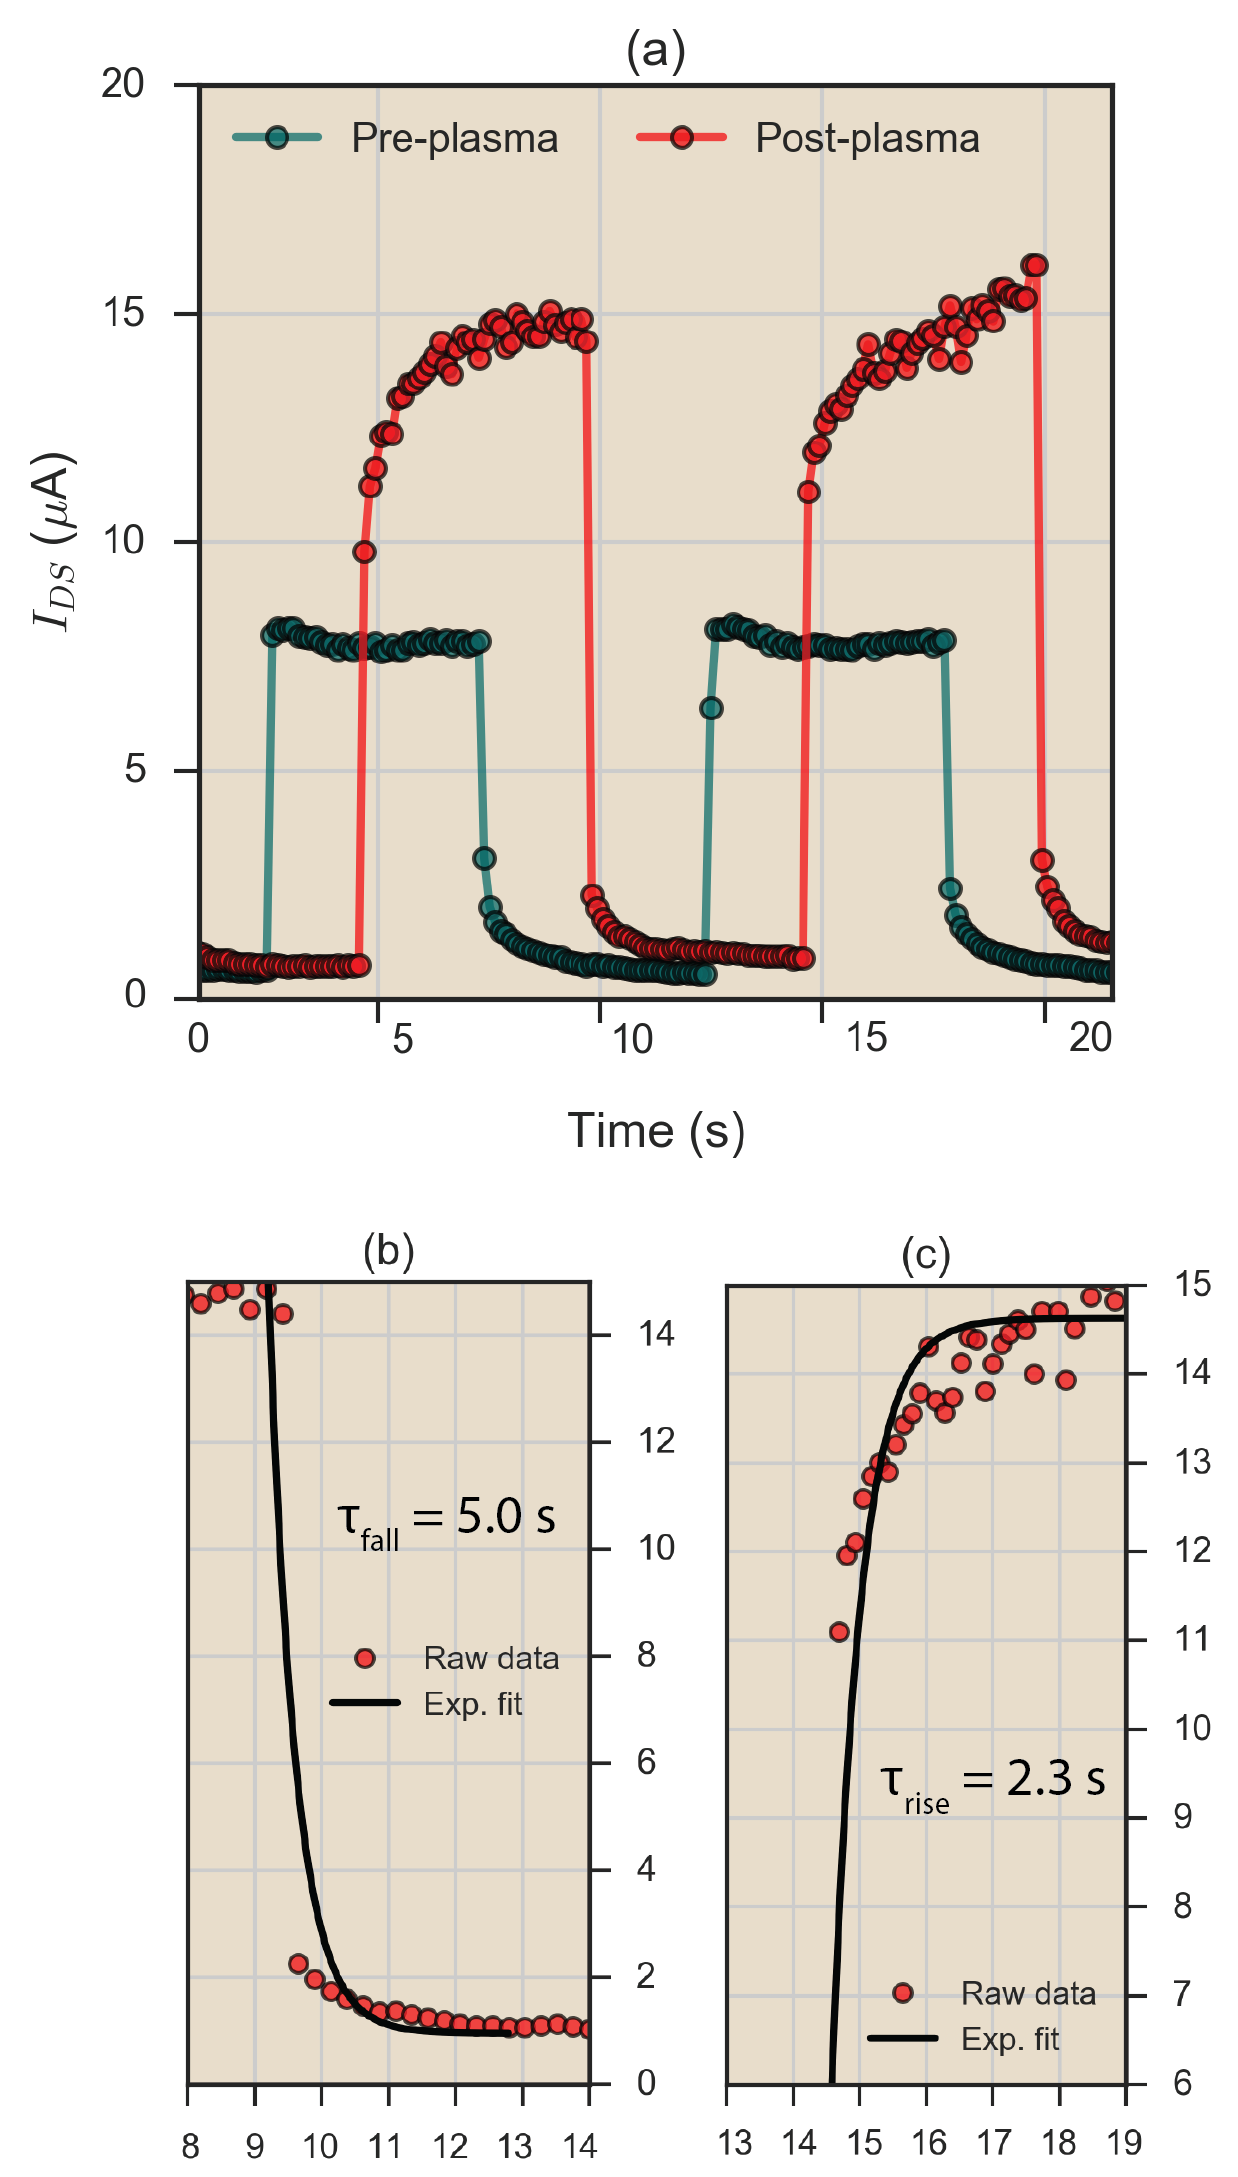
\includegraphics[width=70mm]{Time_response_fig}
\caption{Time response of the device before and after plasma treatment: (a) Comparison of photocurrent response over laser irradiation cycles lasting 5 seconds. (b) Exponential fit of the fall component of the photoresponse for the treated device. (c) Exponential fit of the rise component of the from the next cycle.}
\end{figure}
\end{center}

\indent The temporal response of the monolayer MoS$_2$ phototransistor pre- and post-plasma treatment is charted in Fig. 4(a). The photocurrent is seen to improve two-fold for the tested device when the 632 nm laser irradiation is modulated through 5 sec ON/5 sec OFF cycles at a power of 36 $\mu$W and V$_{DS}$ = 5 V. The post-sensitisation fall ($\tau_{fall}$) and rise ($\tau_{rise}$) times are extracted from single exponential fits in Fig. 4(b) and 4(c) respectively. The time-resolved photoresponses compare favourably with the evaporated MoO$_x$ overlayer report \cite{Yoo2017}, where the rise time at a similar wavelength and much lower irradiation power is 35\% shorter.  \newline
\indent We go on to estimate the level of defectivity in the plasma-treated sample after 2 seconds of exposure. $\frac{1}{f}$ noise measurement have demonstrated the level of charge-trapping sites in monolayer MoS$_2$ varies between $10^{19} - 10^{23}$ eV$^{-1}$ cm$^{-3}$ depending on whether samples are exfoliated or CVD-synthesised \cite{renteria2014low,kim2017analysis}, while the areal trap density for both the mid-gap trap states and band-edge trap states varies in the literature between 10$^{12}$ eV$^{-1}$ cm$^{-2}$ and 10$^{15}$ eV$^{-1}$ cm$^{-2}$ \cite{zhu2014electronic,yuan2017pbti}. The effect of charge traps on carrier transport has been well documented in the case of pristine MoS$_2$ \cite{yu2016realization,yu2017analyzing}, but defect-rich oxygen plasma-treated samples have not been studied in detail to account for the unusual enhanced transport behaviour previously reported \cite{jadwiszczak2017oxide, nan2017improving}. Argon plasma treatment has been shown to increase the amount of electrochemically active surface sites to $\sim 10^{16}$ cm$^{-2}$ \cite{tao2015plasma}, hence we expect the basal plane morphology to be severely affected by the chemical reaction with the plasma. \newline
\indent TEM TEMTEMTEM TEMTEMTE MTE MTEMTEM TEMTE MTEM TEMTE MTEM TEM TEMTEMTEM TEMTEMTE MTE MTEMTEM TEMTE MTEM TEMTE MTEMTEM TEMTEMTEM TEMTEMTE MTE MTEMTEM TEMTE MTEM TEMTE MTEMTEM TEMTEMTEM TEMTEMTE MTE MTEMTEM TEMTE MTEM TEMTE MTEMTEM TEMTEMTEM TEMTEMTE MTE MTEMTEM TEMTE MTEM TEMTE MTEMTEM TEMTEMTEM TEMTEMTE MTE MTEMTEM TEMTE MTEM TEMTE MTEMTEM TEMTEMTEM TEMTEMTE MTE MTEMTEM TEMTE MTEM TEMTE MTEMTEM TEMTEMTEM TEMTEMTE MTE MTEMTEM TEMTE MTEM TEMTE MTEMTEM TEMTEMTEM TEMTEMTE MTE MTEMTEM TEMTE MTEM TEMTE MTEMTEM TEMTEMTEM TEMTEMTE MTE MTEMTEM TEMTE MTEM TEMTE MTEMTEM TEMTEMTEM TEMTEMTE MTE MTEMTEM TEMTE MTEM TEMTE MTEMTEM TEMTEMTEM TEMTEMTE MTE MTEMTEM TEMTE MTEM TEMTE MTEMTEM TEMTEMTEM TEMTEMTE MTE MTEMTEM TEMTE MTEM TEMTE MTEMTEM TEMTEMTEM TEMTEMTE MTE MTEMTEM TEMTE MTEM TEMTE MTEMTEM TEMTEMTEM TEMTEMTE MTE MTEMTEM TEMTE MTEM TEMTE MTEMTEM TEMTEMTEM TEMTEMTE MTE MTEMTEM TEMTE MTEM TEMTE MTEMTEM TEMTEMTEM TEMTEMTE MTE MTEMTEM TEMTE MTEM TEMTE MTEMTEM TEMTEMTEM TEMTEMTE MTE MTEMTEM TEMTE MTEM TEMTE MTEM\newline

\begin{center}
\begin{figure}[!htb]
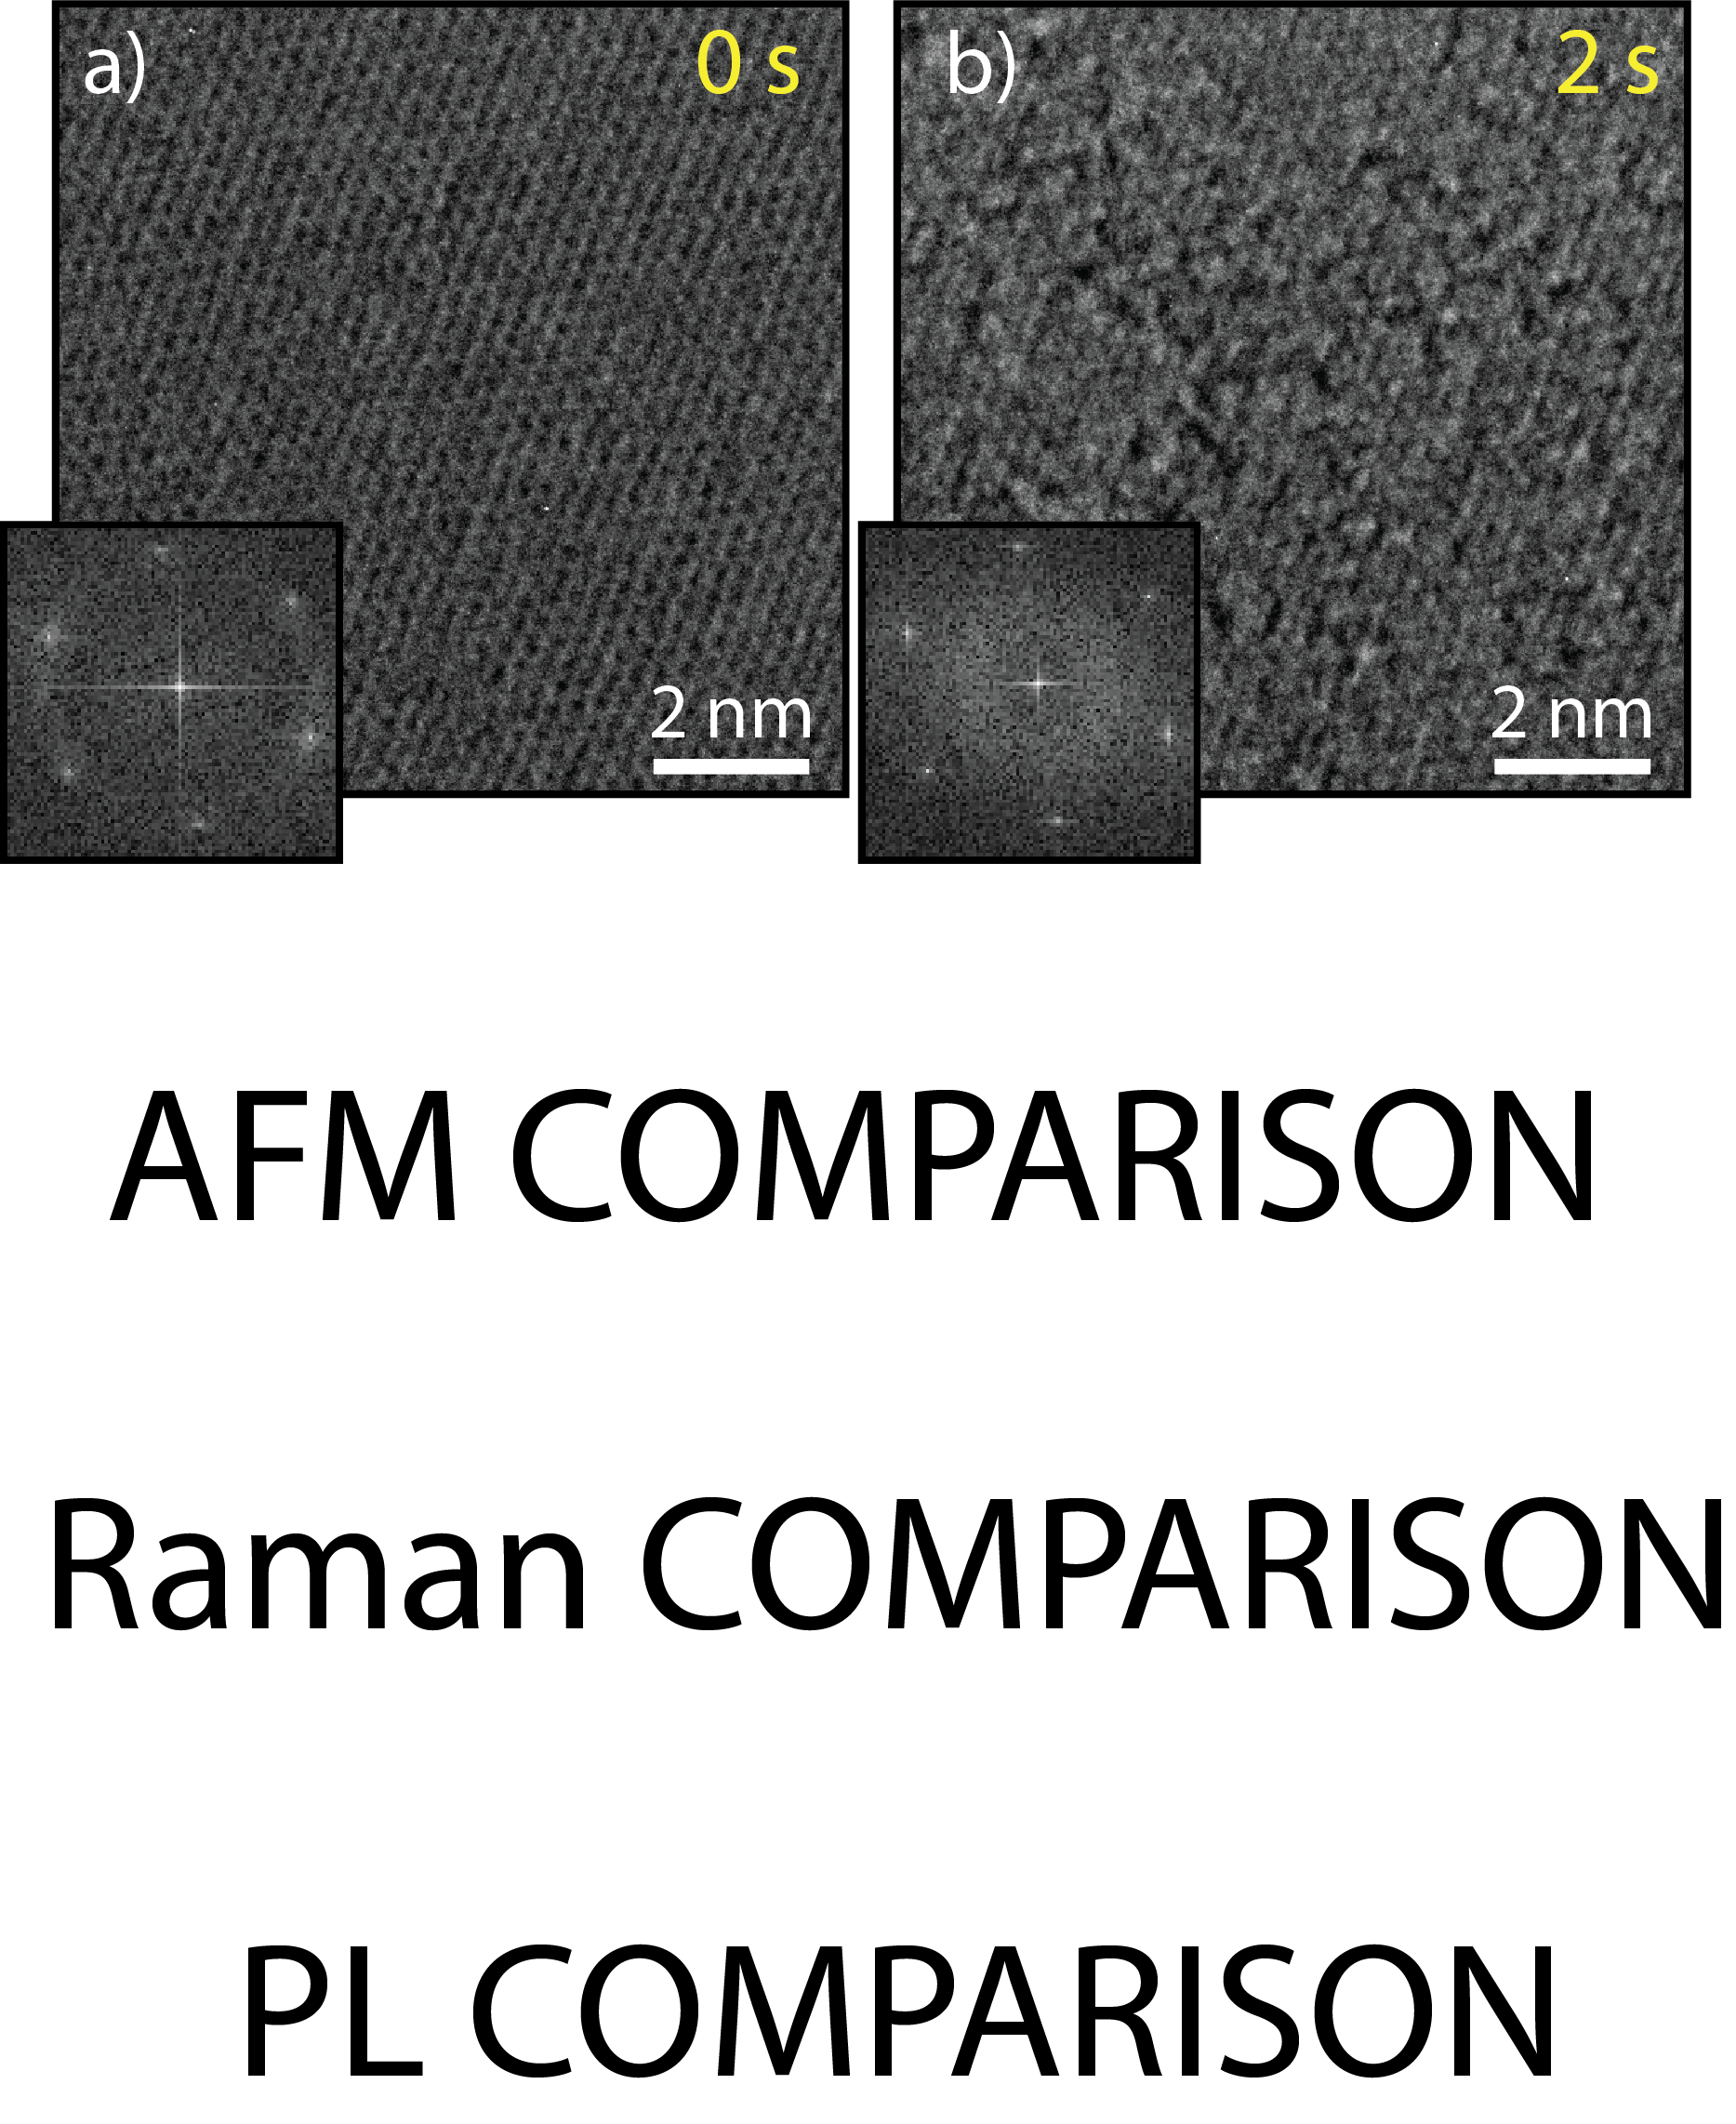
\includegraphics[width=80mm]{Figure_4_photo}
\caption{Characterisation of the plasma-oxidised MoS$_2$ CVD monolayers.}
\end{figure}
\end{center}

\indent AFM AFM AFM AFMAFM AFM AFM AFMAFM AFM AFM AFMAFM AFM AFM AFMAFM AFM AFM AFMAFM AFM AFM AFMAFM AFM AFM AFMAFM AFM AFM AFMAFM AFM AFM AFMAFM AFM AFM AFMAFM AFM AFM AFMAFM AFM AFM AFMAFM AFM AFM AFMAFM AFM AFM AFMAFM AFM AFM AFMAFM AFM AFM AFMAFM AFM AFM AFMAFM AFM AFM AFMAFM AFM AFM AFMAFM AFM AFM AFMAFM AFM AFM AFMAFM AFM AFM AFMAFM AFM AFM AFMAFM AFM AFM AFMAFM AFM AFM AFMAFM AFM AFM AFMAFM AFM AFM AFMAFM AFM AFM AFMAFM AFM AFM AFMAFM AFM AFM AFMAFM AFM AFM AFMAFM AFM AFM AFMAFM AFM AFM AFMAFM AFM AFM AFMAFM AFM AFM AFMAFM AFM AFM AFMAFM AFM AFM AFMAFM AFM AFM AFMAFM AFM AFM AFMAFM AFM AFM AFMAFM AFM AFM AFMAFM AFM AFM AFMAFM AFM AFM AFMAFM AFM AFM AFMAFM AFM AFM AFMAFM AFM AFM AFMAFM AFM AFM AFMAFM AFM AFM AFMAFM AFM AFM AFMAFM AFM AFM AFMAFM AFM AFM AFMAFM AFM AFM AFMAFM AFM AFM AFMAFM AFM AFM AFMAFM AFM AFM AFMAFM AFM AFM AFMAFM AFM AFM AFMAFM AFM AFM AFMAFM AFM AFM AFMAFM AFM AFM AFMAFM AFM AFM AFMAFM AFM AFM AFMAFM AFM AFM AFMAFM AFM AFM AFM \newline
\indent RAMAN RAMAN RAMANA RAMANARAMAN RAMAN RAMANA RAMANARAMAN RAMAN RAMANA RAMANARAMAN RAMAN RAMANA RAMANARAMAN RAMAN RAMANA RAMANARAMAN RAMAN RAMANA RAMANARAMAN RAMAN RAMANA RAMANARAMAN RAMAN RAMANA RAMANARAMAN RAMAN RAMANA RAMANARAMAN RAMAN RAMANA RAMANARAMAN RAMAN RAMANA RAMANARAMAN RAMAN RAMANA RAMANARAMAN RAMAN RAMANA RAMANARAMAN RAMAN RAMANA RAMANARAMAN RAMAN RAMANA RAMANARAMAN RAMAN RAMANA RAMANARAMAN RAMAN RAMANA RAMANARAMAN RAMAN RAMANA RAMANARAMAN RAMAN RAMANA RAMANARAMAN RAMAN RAMANA RAMANARAMAN RAMAN RAMANA RAMANARAMAN RAMAN RAMANA RAMANARAMAN RAMAN RAMANA RAMANARAMAN RAMAN RAMANA RAMANARAMAN RAMAN RAMANA RAMANARAMAN RAMAN RAMANA RAMANARAMAN RAMAN RAMANA RAMANARAMAN RAMAN RAMANA RAMANARAMAN RAMAN RAMANA RAMANARAMAN RAMAN RAMANA RAMANARAMAN RAMAN RAMANA RAMANARAMAN RAMAN RAMANA RAMANARAMAN RAMAN RAMANA RAMANARAMAN RAMAN RAMANA RAMANARAMAN RAMAN RAMANA RAMANARAMAN RAMAN RAMANA RAMANARAMAN RAMAN RAMANA RAMANARAMAN RAMAN RAMANA RAMANARAMAN RAMAN RAMANA RAMANARAMAN RAMAN RAMANA RAMANARAMAN RAMAN RAMANA RAMANARAMAN RAMAN RAMANA RAMANARAMAN RAMAN RAMANA RAMANARAMAN RAMAN RAMANA RAMANARAMAN RAMAN RAMANA RAMANARAMAN RAMAN RAMANA RAMANARAMAN RAMAN RAMANA RAMANARAMAN RAMAN RAMANA RAMANARAMAN RAMAN RAMANA RAMANARAMAN RAMAN RAMANA RAMANARAMAN RAMAN RAMANA RAMANARAMAN RAMAN RAMANA RAMANARAMAN RAMAN RAMANA RAMANA \newline
\indent PL PL PL PL PL PL PL PL PL PL PL PL PL PL PL PL PL PL PL PL PL PL PL PL PL PL PL PL PL PL PL PL PL PL PL PL PL PL PL PL PL PL PL PL PL PL PL PL PL PL PL PL PL PL PL PL PL PL PL PL PL PL PL PL PL PL PL PL PL PL PL PL PL PL PL PL PL PL PL PL PL PL PL PL PL PL PL PL PL PL PL PL PL PL PL PL PL PL PL PL PL PL PL PL PL PL PL PL PL PL PL PL PL PL PL PL PL PL PL PL PL PL PL PL PL PL PL PL PL PL PL PL PL PL PL PL PL PL PL PL PL PL PL PL PL PL PL PL PL PL PL PL PL PL PL PL PL PL PL PL PL PL PL PL PL PL PL PL PL PL PL PL PL PL PL PL PL PL PL PL PL PL PL PL PL PL PL PL PL PL PL PL PL PL PL PL PL PL PL PL PL PL PL PL PL PL PL PL PL PL PL PL PL PL PL PL PL PL PL PL PL PL PL PL PL PL PL PL PL PL PL PL PL PL PL PL PL PL PL PL PL PL PL PL PL PL PL PL PL PL PL PL PL PL PL PL PL PL PL PL PL PL PL PL PL PL \newline
\indent The physical process responsible for the reported photoresponsivity improvement in plasma-treated MoS$_2$ has been proposed as the resultant carrier trapping at the now-doped MoS$_2$/metal interface \cite{wi2014enhancement}, and more appropriately in this case, the pristine MoS$_2$/MoO$_x$ interface \cite{Yoo2017}.
The electron affinity and band gap of monolayer MoS$_2$ are ~ 4.3 eV and 1.2 eV respectively \cite{Liang2013,Mak2010a}. After the rapid plasma treatment, MoO$_x$ is generated in the device as demonstrated in the previous discussion. MoO$_x$ is commonly known as a high work function (6.8 eV) material with a band gap of 3 eV.\cite{Kang2014, Yoo2017} In the presently studied device, plasma-generated oxides and unreacted MoS$_2$ will form an effective medium that spans the FET channel. As the Fermi
level of MoS$_2$ is higher than that of MoO$_x$, significant band bending will occur at the interface as seen in Fig. 4. After reaching equilibrium, the built-in electric field gradient will be directed from MoS$_2$ to MoO$_x$. Photo-generated holes will become trapped at the material interface inhibiting electron-hole recombination, and thereby enhancing the measured
photocurrent. Hence, the responsivity of the device to laser irradiation is improved, as any photo-generated electrons in the plasma-treated system are free to move in the channel without direct recombination with holes. \\

\indent In conclusion, we have demonstrated that the photoresponsivity of MoS$_2$ monolayer FETs can be enhanced two-fold by the introduction of surface-bound molybdenum oxide. We confirm the presence of MoO$_x$ induced by plasma treatment using TEM, AFM, Raman and PL spectroscopy. The effect of the mobility enhancement and photoresponsivity was also noted to depend on laser power and be more prominent at powers exceeding several $\mu$Watts. Our work can provide insight into heterostructure physics in novel nano-devices in the areas of optoelectronics and 2D layered materials. 

%\begin{center}
%\begin{figure}[!htb]
%\includegraphics[width=80mm]{E}
%\caption{Energy band digram of the system consist of pristine MoS$_2$ plasma generated MoO$_x$.}
%\end{figure}
%\end{center}




\section*{Acknowledgements}

We are grateful to members of staff at the Advanced Microscopy Laboratory, CRANN, Trinity College Dublin for their continued technical support. We thank Jian-Yao Zheng for assistance with the laser set-up and Chuan Zhong for help with film deposition. We would like to acknowledge support from the following funding bodies: GRANT NUMBERS.



\bibliographystyle{apsrev}
\bibliography{my}
 
\end{document}
% ****** End of file apssamp.tex ******
